\documentclass[10pt,a4paper]{article}
\usepackage[utf8]{inputenc}
\usepackage[T1]{fontenc}
\usepackage[ngerman]{babel}
\usepackage{amsmath}
\usepackage{amsfonts}
\usepackage{amssymb}
\usepackage{graphicx}


\author{Gruppe 02}
\title{Pflichtenheft}
\begin{document}

	\subsection{Adminbereich}
	\subsubsection{Benutzer sperren}
	\begin{figure}[h]
		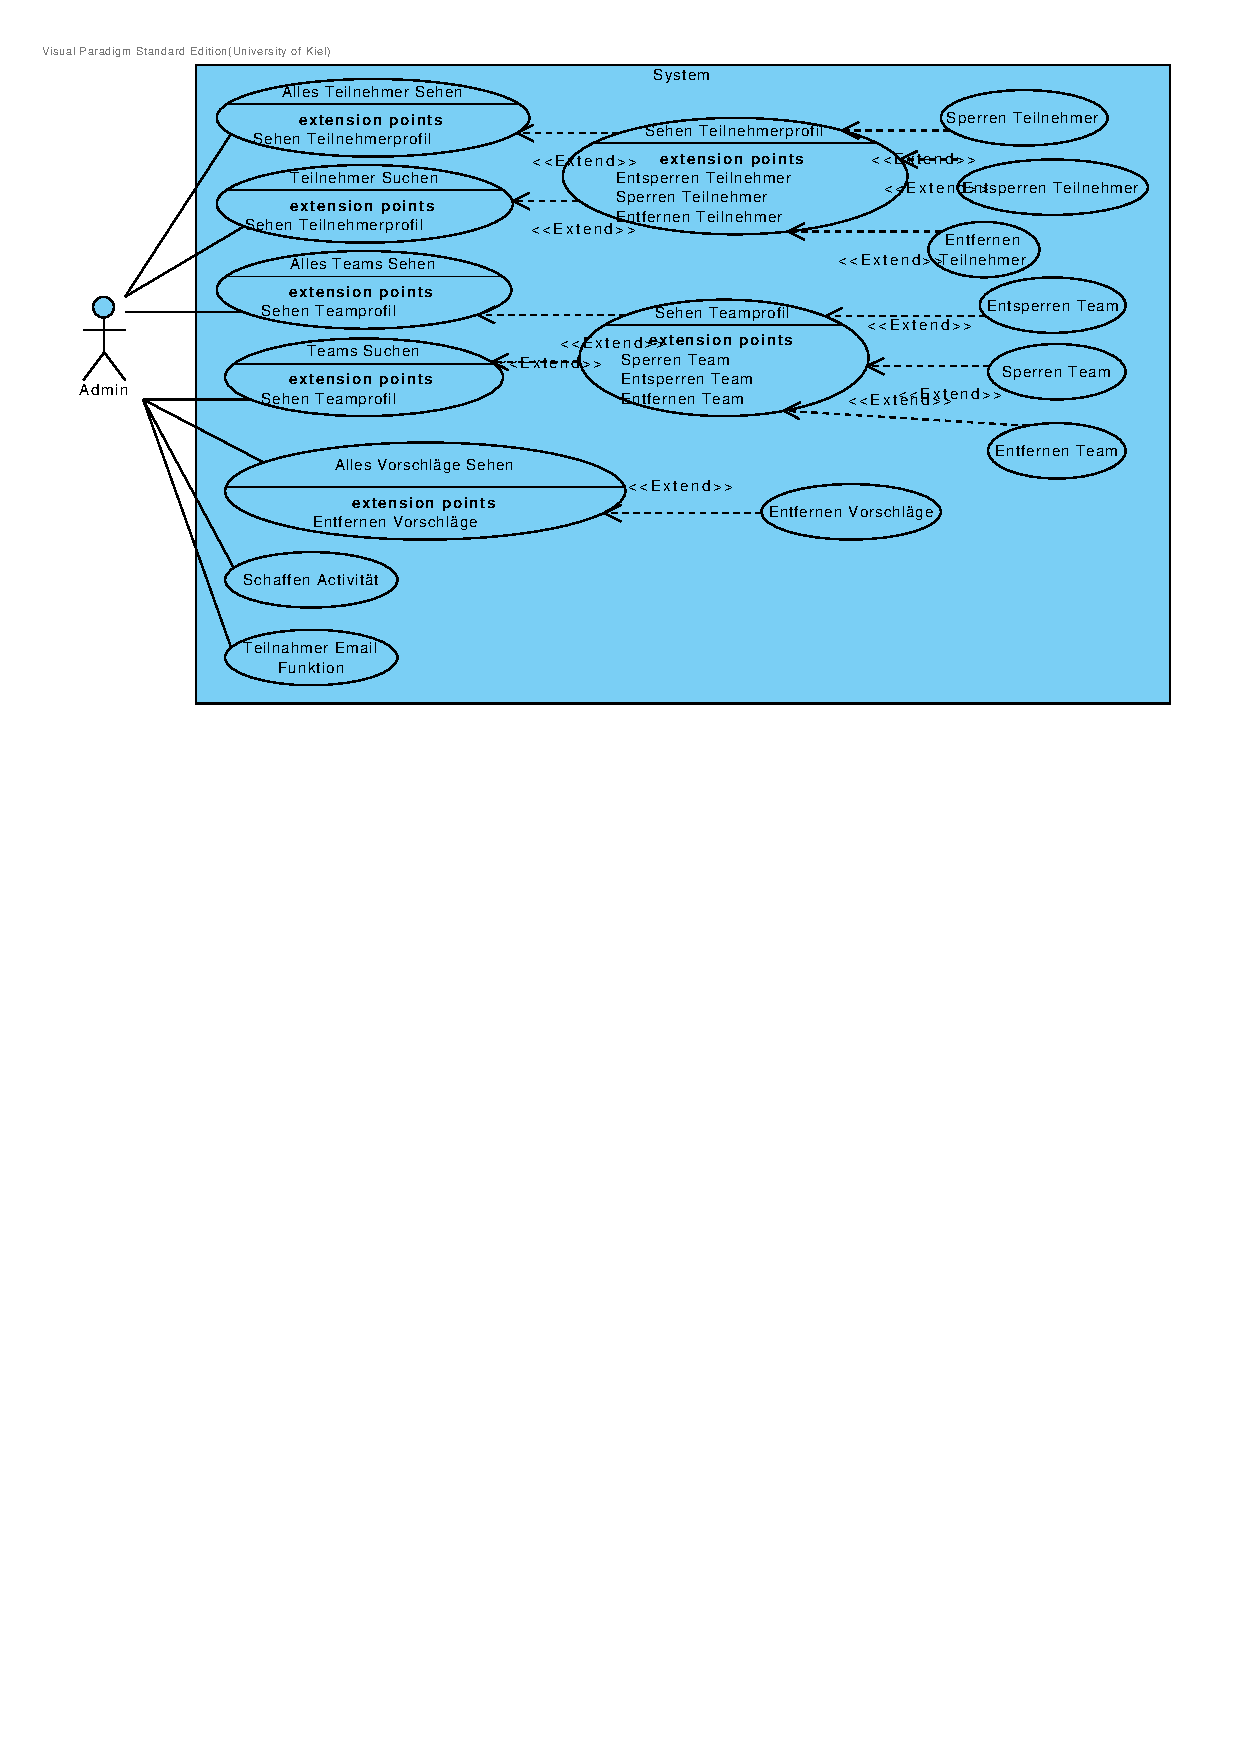
\includegraphics[width=\linewidth]{gfx/webseite/adminbereich.pdf}
	\end{figure}
	\begin{tabular}{|l|p{.5\linewidth}|}
	\hline Use Case Nummer & 1.7.1 \\ 
	\hline Use Case Name & Benutzer sperren \\ 
	\hline Initiierender Akteur & Admin \\
	\hline Weitere Akteure & Benutzer \\
	\hline Kurzbeschreibung & Der Admin w\"ahlt einen Benutzer aus und sperrt ihn, sodass dieser nicht mehr auf die Anwendung zugreifen kann \\
	\hline Vorbedingung & Administrator ist als solcher angemeldet \\
	\hline Nachbedingung & Das Profil des ausgew\"ahlten Benutzers ist gesperrt \\
	\hline \multicolumn{2}{|c|}{Funktionalit\"at des Use Cases}\\
	\hline Ablauf & \begin{itemize}
			\item Admin sucht den zu sperrenden Benutzer raus\\
			\item Admin w\"ahlt Benutzer sperren aus\\
			\item Admin best\"atigt die Entscheidung den Benutzer zu sperren\\
		\end{itemize} \\
	\hline Alternativen & - \\
	\hline Ausnahmen & - \\
	\hline Benutzte Use Cases & \begin{itemize}
			\item Benutzerliste einsehen\\
			\item Benutzer suchen\\
			\item Benutzerprofil ansehen\\
		\end{itemize} \\
	\hline \multicolumn{2}{|c|}{Weitere Informationen} \\
	\hline Spezielle Anforderungen &  \\
	\hline Annahmen &  \\
	\hline
	\end{tabular}
	
	\subsubsection{Benutzer reaktivieren}
	\begin{tabular}{|l|p{.5\linewidth}|}
	\hline Use Case Nummer & 1.7.2 \\ 
	\hline Use Case Name & Benutzer reaktivieren \\ 
	\hline Initiierender Akteur & Admin \\
	\hline Weitere Akteure & Benutzer \\
	\hline Kurzbeschreibung & Der Admin w\"ahlt einen zur Zeit gesperrten Benutzer aus und reaktiviert ihn, sodass dieser wieder Zugriff auf die Anwendung hat \\
	\hline Vorbedingung & Administrator als solcher angemeldet \\
	\hline Nachbedingung & Der reaktivierte Benutzer hat wieder vollen Zugriff auf die Anwendung und sein Profil ist f\"ur andere wieder einsehbar \\
	\hline \multicolumn{2}{|c|}{Funktionalit\"at des Use Cases}\\
	\hline Ablauf & \begin{itemize}
			\item Admin w\"ahlt einen gesperrten Benutzer aus\\
			\item Der Admin reaktiviert den entsprechenden Benutzer\\
			\item Der Admin best\"atigt, dass er diesen Benutzer wirklich reaktivieren m\"ochte\\
		\end{itemize} \\
	\hline Alternativen & \\
	\hline Ausnahmen &  \\
	\hline Benutzte Use Cases & \begin{itemize}
			\item Benutzerliste einsehen\\
			\item Benutzerprofil ansehen\\
		\end{itemize} \\
	\hline \multicolumn{2}{|c|}{Weitere Informationen} \\
	\hline Spezielle Anforderungen &  \\
	\hline Annahmen &  \\
	\hline
	\end{tabular}
	
	\subsubsection{Benutzer l\"oschen}
	\begin{tabular}{|l|p{.5\linewidth}|}
	\hline Use Case Nummer & 1.7.3 \\ 
	\hline Use Case Name & Benutzer l\"oschen \\ 
	\hline Initiierender Akteur & Admin \\
	\hline Weitere Akteure & User \\
	\hline Kurzbeschreibung & Der Administrator w\"ahlt einen Benutzer aus und l\"oscht diesen komplett aus dem System \\
	\hline Vorbedingung & Administrator ist als solcher angemeldet \\
	\hline Nachbedingung & Das Profil des gel\"oschten Teilnehmers ist aus dem System entfernt \\
	\hline \multicolumn{2}{|c|}{Funktionalit\"at des Use Cases}\\
	\hline Ablauf & \begin{itemize}
			\item Admin w\"ahlt den zu l\"oschenden Benutzer aus\\
			\item Der Admin l\"oscht den betreffenden Benutzer\\
			\item Der Admin best\"atigt, dass er den Benutzer wirklich l\"oschen m\"ochte\\
		\end{itemize} \\
	\hline Alternativen & Der Admin sucht den zu l\"oschenden Benutzer \"uber die Suchfunktion\\
	\hline Ausnahmen &  \\
	\hline Benutzte Use Cases & \begin{itemize}
			\item Benutzerliste einsehen\\
			\item Benutzer suchen
			\item Benutzerprofil einsehen\\
		\end{itemize} \\
	\hline \multicolumn{2}{|c|}{Weitere Informationen} \\
	\hline Spezielle Anforderungen &  \\
	\hline Annahmen &  \\
	\hline
	\end{tabular} 
	
	\subsubsection{Team l\"oschen}
	\begin{tabular}{|l|p{.5\linewidth}|}
	\hline Use Case Nummer & 1.7.4 \\ 
	\hline Use Case Name & Team l\"oschen \\ 
	\hline Initiierender Akteur & Admin \\
	\hline Weitere Akteure & User \\
	\hline Kurzbeschreibung & Der Administrator hat die M\"oglichkeit ein Team zu l\"oschen, wobei die einzelnen Mitglieder jedoch nicht automatisch gel\"oscht werden \\
	\hline Vorbedingung & Als Administrator angemeldet \\
	\hline Nachbedingung & Das Team wurde aus dem System entfernt, die einzelnen Benutzer sind noch vorhanden, jedoch nun ohne Teamzugeh\"origkeit \\
	\hline \multicolumn{2}{|c|}{Funktionalit\"at des UseCases}\\
	\hline Ablauf & \begin{itemize}
			\item Admin w\"ahlt das zu l\"oschende Team aus\\
			\item Der Admin l\"oscht das Team\\
			\item Der Admin best\"atigt, dass er das ausgew\"ahlte Team wirklich l\"oschen m\"ochte\\
		\end{itemize} \\
	\hline Alternativen & Alternativ kann der Admin das Team \"uber die Suche finden \\
	\hline Ausnahmen &  \\
	\hline Benutzte Use Cases & \begin{itemize}
			\item Teamliste einsehen\\
			\item Team suchen\\
			\item Teamprofil einsehen\\
		\end{itemize} \\
	\hline \multicolumn{2}{|c|}{Weitere Informationen} \\
	\hline Spezielle Anforderungen &  \\
	\hline Annahmen &  \\
	\hline
	\end{tabular}
	
	\subsubsection{Vorschlag in Aktivit\"at umwandeln}
	\begin{tabular}{|l|p{.5\linewidth}|}
	\hline Use Case Nummer & 1.7.5 \\ 
	\hline Use Case Name & Vorschlag in Aktivit\"at umwandeln \\ 
	\hline Initiierender Akteur & Admin \\
	\hline Weitere Akteure & \\
	\hline Kurzbeschreibung & Der Admin kann einen besonders guten Vorschlag in eine Aktivit\"at umwandeln, die dann allen Benutzern zur Verf\"ugung steht \\
	\hline Vorbedingung & Als Administrator angemeldet \\
	\hline Nachbedingung & Der umgewandelte Vorschlag ist nicht mehr bei den Vorschl\"agen aufgef\"uhrt, daf\"ur jedoch in der Aktivit\"atenliste \\
	\hline \multicolumn{2}{|c|}{Funktionalit\"at des UseCases}\\
	\hline Ablauf & \begin{itemize}
			\item Der Admin w\"ahlt den Vorschlag aus, den er zu einer Aktivit\"at ab\"andern m\"ochte
			\item Der Admin tr\"agt die noch ben\"otigten Informationen in die Bearbeitungsmaske ein und speichert die Aktivit\"at
		\end{itemize} \\
	\hline Alternativen &  \\
	\hline Ausnahmen & \begin{itemize}
			\item Der Vorgang kann nicht abgeschlossen werden, wenn nicht alle ben\"otigten Informationsfelder ausgef\"ullt sind\\
			\item Der Vorgang kann nicht abgeschlossen werden, wenn der eingegebene Titel oder Beschreibungstext zu lang sind\\
			\item Der Vorgang kann nicht abgeschlossen werden, wenn der eingegebene Punktwert kein Integer zwischen 1 und 5 ist\\
		\end{itemize} \\
	\hline Benutzte Use Cases &  \\
	\hline \multicolumn{2}{|c|}{Weitere Informationen} \\
	\hline Spezielle Anforderungen &  \\
	\hline Annahmen & Der Admin achtet darauf, dass die Eingaben korrekt und sinnvoll sind \\
	\hline
	\end{tabular}
	
	\subsubsection{Vorschlag l\"oschen}
	\begin{tabular}{|l|p{.5\linewidth}|}
	\hline Use Case Nummer & 1.7.6 \\ 
	\hline Use Case Name & Vorschlag l\"oschen \\ 
	\hline Initiierender Akteur & Admin \\
	\hline Weitere Akteure & \\
	\hline Kurzbeschreibung & Der Administrator w\"ahlt einen unpassenden oder anderweitig \"uberfl\"ussigen Vorschlag aus und l\"oscht diesen \\
	\hline Vorbedingung & Als Administrator angemeldet \\
	\hline Nachbedingung & Der Vorschlag erscheint auf der Vorschlagsseite nicht mehr und ist aus dem System gel\"oscht \\
	\hline \multicolumn{2}{|c|}{Funktionalit\"at des UseCases}\\
	\hline Ablauf & \begin{itemize}
			\item Admin w\"ahlt den zu l\"oschenden Vorschlag aus\\
			\item Der Admin best\"atigt, dass er den Vorschlag l\"oschen m\"ochte\\
		\end{itemize} \\
	\hline Alternativen &  \\
	\hline Ausnahmen &  \\
	\hline Benutzte Use Cases & Vorschlagsliste ansehen\\
	\hline \multicolumn{2}{|c|}{Weitere Informationen} \\
	\hline Spezielle Anforderungen &  \\
	\hline Annahmen &  \\
	\hline
	\end{tabular}
	
	\subsubsection{neue Aktivit\"at erzeugen}
	\begin{tabular}{|l|p{.5\linewidth}|}
		\hline Use Case Nummer & 1.7.7 \\ 
		\hline Use Case Name & neue Aktivit\"at erzeugen \\ 
		\hline Initiierender Akteur & Admin \\
		\hline Weitere Akteure & \\
		\hline Kurzbeschreibung & Der Administrator f\"ugt der Liste der verf\"ugbaren Aktivit\"aten eine neue hinzu (nicht notwendigerweise vorher als Vorschlag vorhanden) \\
		\hline Vorbedingung & Als Administrator angemeldet \\
		\hline Nachbedingung & Die Aktivit\"atenliste ist um eine Aktivit\"at erweitert \\
		\hline \multicolumn{2}{|c|}{Funktionalit\"at des UseCases}\\
		\hline Ablauf & \begin{itemize}
			\item Admin w\"ahlt auf der Aktivit\"atenseite "neue Aktivit\"at hinzuf\"ugen"\\
			\item Der Admin f\"ullt das entsprechende Formular mit den ben\"otigten Informationen aus\\
			\item Der Admin speichert die neue Aktivit\"at\\
		\end{itemize} \\
		\hline Alternativen &  \\
		\hline Ausnahmen & Falsche Eingaben sorgen daf\"ur, dass die Aktivit\"at nicht gespeichert werden kann \\
		\hline Benutzte Use Cases & Aktivit\"atenliste ansehen\\
		\hline \multicolumn{2}{|c|}{Weitere Informationen} \\
		\hline Spezielle Anforderungen &  \\
		\hline Annahmen & Der Admin f\"ullt das Formular korrekt und sinnvoll aus \\
		\hline
	\end{tabular}
	
	\subsubsection{Alle Benutzer per E-Mail benachrichtigen}
	\begin{tabular}{|l|p{.5\linewidth}|}
		\hline Use Case Nummer & 1.7.8 \\ 
		\hline Use Case Name & Alle Benutzer per E-Mail benachrichtigen \\ 
		\hline Initiierender Akteur & Admin \\
		\hline Weitere Akteure & Benutzer \\
		\hline Kurzbeschreibung & Der Administrator hat die M\"oglichkeit alle Benutzer per Mail zu kontaktieren (f\"ur Hinweise bzgl. Challenges etc.) \\
		\hline Vorbedingung & Als Administrator angemeldet \\
		\hline Nachbedingung & - \\
		\hline \multicolumn{2}{|c|}{Funktionalit\"at des UseCases}\\
		\hline Ablauf & \begin{itemize}
			\item Admin w\"ahlt bei seinen Optionen "Nachricht an alle Benutzer"\\
			\item Der Admin f\"ullt das entsprechende Formular mit der Nachricht aus\\
			\item Der Admin verschickt die Nachricht automatisch per Rundmail an alle Teilnehmer\\
		\end{itemize} \\
		\hline Alternativen &  \\
		\hline Ausnahmen & \\
		\hline Benutzte Use Cases & \\
		\hline \multicolumn{2}{|c|}{Weitere Informationen} \\
		\hline Spezielle Anforderungen &  \\
		\hline Annahmen &  \\
		\hline
	\end{tabular}
	
\end{document}